\documentclass[11pt]{jsarticle}

\usepackage{SPR}

\headerSPR
\begin{document}
	\titleSPR{\number\year}{\number\month}{\number\day}{D1}{吉田 皓太郎}
%%%%%%%%%%%%%%%%%%%%%%%%%%%%%%%%%%%%%%
	\articleSPRabst
		\begin{itemize}
			\item 着後形状を評価可能なバストモデルの構築.
		\end{itemize}
		
		
	\articleSPRobj
		\begin{enumerate}
			\item カップ装着時における,着後形状が分かればよい.(着圧に関してはバストよりもベルトの話?の方が大きな要素となる)
			\item そこまでのたくさんの正確なデータを必要としない.
		\end{enumerate}
%%%%%%%%%%%%%%%%%%%%%%%%%%%%%%%%%%%%%%
% 1.前回からのノルマ
	\articleSPRitemsone
		%\begin{enumerate}
		%	\item A
		%\end{enumerate}
		
		\tableofcontents
		
		
%%%%%%%%%%%%%%%%%%%%%%%%%%%%%%%%%%%%%%
%\begin{itemize}
%	\item 新規手法について
%	\item ISFAアウトライン
%\end{itemize}
%%%%%%%%%%%%%%%%%%%%%%%%%%%%%%%%%%%%%%
% 2.具体的な成果
	\articleSPRitemstwo
%%%%%%%%%%%%%%%%%%%%%%%%%%%%%%%%%%%%%%
	\section{布物性検証実験について}
		\begin{figure}[thpb]
			\begin{minipage}{0.5\hsize}
				\centering
				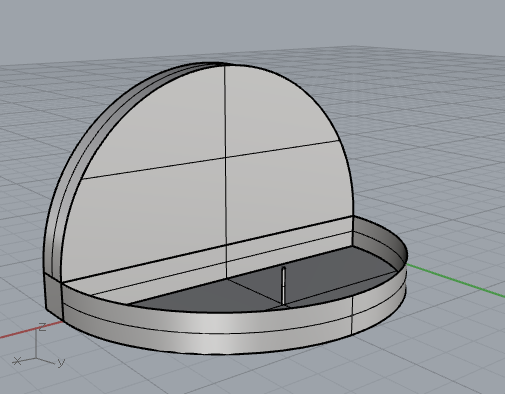
\includegraphics[width = 0.6\columnwidth]{./figure/ExperimentDevice.png}
				\caption{in perspective view}
			\end{minipage}
			\begin{minipage}{0.5\hsize}
				\centering
				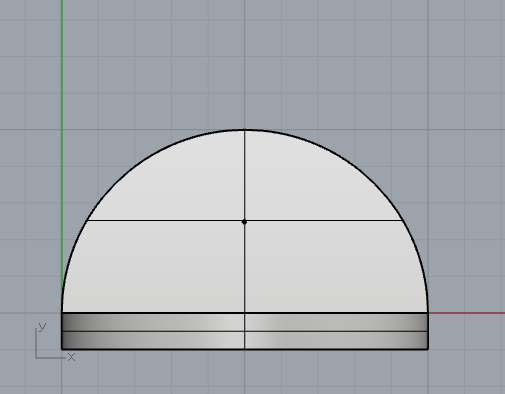
\includegraphics[width = 0.6\columnwidth]{./figure/ExperimentDevice_xyview.png}
				\caption{in $ x-y $ view}
			\end{minipage}
			\begin{minipage}{0.5\hsize}
				\centering
				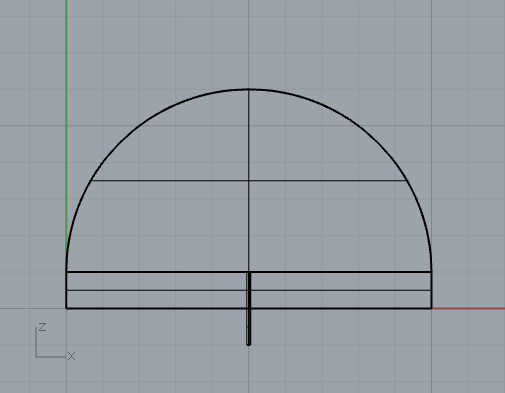
\includegraphics[width = 0.6\columnwidth]{./figure/ExperimentDevice_zxview.png}
				\caption{in $ x-z $ view}
			\end{minipage}
			\begin{minipage}{0.5\hsize}
				\centering
				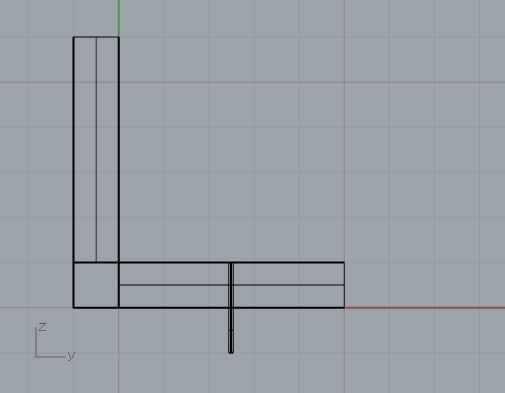
\includegraphics[width = 0.6\columnwidth]{./figure/ExperimentDevice_yzview.png}
				\caption{in $ y-z $ view}
			\end{minipage}
			\caption{Shape of Experiment Device}
		\end{figure}
		この物性による実験検証を以下の手順で進めてみたいと思う.まず布の機械的特性をそのまま線形弾性体として扱うことは難しいと考えられるため,伸縮しやすく扱いやすいものとして,シリコンゴムなどがよいのではないかと思われる.
		
		今回では,ワイヤおよび上下接ぎラインが変化しないものとするため,十分にかたい剛体によってこの二つを作成する.この二つのラインは互いに円弧であるとし,その上で図に示すような検証用装置をCAD(Rhinoceros)によって設計し,3Dプリンタを用いて作成する.円の片方には,空気を入れる穴をあけてある.
		
		次に実験手順について述べる.
		\begin{enumerate}
			\item 作成したデバイスの空いている部分をゴムなどの対象物質で覆う.
			\item 最初の装置全体の質量を計測
			\item 適当な理想気体に従う気体$ G $を用意し,空気穴から気体を挿入する.
			\item 質量を計測することで,挿入前後の質量変化$ \Delta M $を求める.
			\item 内部圧力$ \hat{p} $を求める.
			\item 対象物質の物性と圧力$ \hat{p} $を用いて計算した形状と,気体を入れて膨らませた実物を計測・比較する.
		\end{enumerate}
	
		この内部圧力$ \hat{p} $は挿入の過程で等温過程であるとすれば,ボイル-シャルルの法則により次式で表される.
		\begin{equation}\label{eq:boil}
			\hat{p}(V_0 + \Delta V) = p_0 V_0
		\end{equation}
		$ p_0 $は大気圧と等しいとし,$ V_0 $は元の可展面状態の体積である.この$ V_0 $は$ x=r\sin \theta $で切った際の切り口が常に三角形であることから$ V_0 = \frac{2}{3} r^3$で求められ,$ \Delta V $は$ G $の気体密度が$ \rho$ならば$ \Delta V  = \frac{\Delta M}{\rho}$で求められる.
		以上により,この$ \hat{p} $を与えられたデータによって表現すると次式のようにあらわされる.
		\begin{equation}\label{eq:PressEq}
			\hat{p} = \frac{2 r^3 \rho}{2 r^3 \rho + 3 \Delta M} p_0
		\end{equation}
		
		現在は,石原が3Dプリンタを使う用事がたくさんあるとのことなので,実際に制作し取り掛かるのは帰国後になるかと思います.
	\section{ISFAについて}
		最終章に関して相談があります.検証の章で次の一文「We confirmed our proposed method by reproducing the cup shape from its data points which imitate cup shape made of developable surface.」なのですが,自分の中でいまひとつであると思っております.
		
		私の中では,手法が正しいということは,可展面を二枚貼り合わせた形状の三次元点群を同じように二枚の可展面で再現することができるはずであるという論旨なのですが,なかなか一文では分かりづらいかなと感じております.何かうまくまとめることができないかと相談したいです.
		
		なお,texファイルにはすでにすべて直してある状態です.
	\section{ABAQUSについて}
		追加トークンに関する処理待ち	
		
	
	\newpage
\vspace{10cm}
%%%%%%%%%%%%%%%%%%%%%%%%%%%%%%%%%%%%%%
% 3.達成できなかったこととその問題点
	%\articleSPRthree
%%%%%%%%%%%%%%%%%%%%%%%%%%%%%%%%%%%%%%

\vspace{14cm}
%%%%%%%%%%%%%%%%%%%%%%%%%%%%%%%%%%%%%%
	\articleSPRfour
	\articleSPRfive
\end{document}
